\chapter[A PROPOSTA]{A PROPOSTA}

Este capítulo apresenta a proposta do trabalho de conclusão de curso, exibindo detalhes da implementação a ser realizada.

\section{Introdução}
Avanços tecnológicos e a criação de linguagens de programação, diferentes técnicas e paradigmas e outros conceitos relacionados ao desenvolvimento de software contribui para que a necessidade de interação entre estes elementos seja emergente, de modo a viabilizar a construção de sistemas cada vez mais robustos e inteligentes. Esta interação entre elementos de software não consistem de aplicações robustas que executam todas as suas atividades de forma independente de outras aplicações: cada vez mais, diversos sistemas de software interagem com outros, podendo ser estes desenvolvidos tomando como base outros paradigmas ou escritos em outras linguagens de programação e utilizando-se diferentes técnicas.

A fim de suprir esta necessidade de interação entre sistemas diversos, foi criado um modelo arquitetural conhecido como Arquitetura Baseada em Serviços (ou \textit{Service-Oriented Architecture} - SOA). Este modelo arquitetural utiliza o conceito de serviço como uma unidade que representa uma funcionalidade do sistema, além de trazer consigo os conceitos de interoperabilidade, flexibilidade e baixo acoplamento entre os diversos sistemas ou serviços.

Para este trabalho de conclusão de curso, a proposta consiste em desenvolver uma arquitetura baseada no modelo SOA para um ambiente virtual, propiciando que diversos trabalhos já desenvolvidos e também aqueles em desenvolvimento não sejam mais "engavetados". Por meio do uso do modelo SOA, será possível integrar tais aplicações, ou serviços nos moldes dos termos de SOA, de modo que estas possam trocar dados e fazer uso do serviço disponibilizado por outras, indepentemente das tecnologias utilizadas para o desenvolvimento das mesmas. Também faz parte da proposta, o estabelecimento de um protocolo de comunicação entre as aplicações, bem como o padrão de comunicação a ser utilizado.

Desta forma, será viável a disponibilização à sociedade de uma plataforma virtual que conterá os trabalhos realizados dentro da universidade, sejam oriundos de projetos de conclusão de curso, disciplinas ou projetos de extensão e pesquisa.

\section{Proposta de arquitetura}

\subsection{Requisitos}
A partir da necessidade identificada de disponibilizar aplicações que foram desenvolvidas, bem como aquelas que estão em desenvolvimento e que serão desenvolvidas, através de uma plataforma virtual único, algumas das principais características arquiteturais deste ambiente que influenciaram na escolha do modelo arquitetural para a construção da plataforma são:

\begin{itemize}
\item A comunicação entre as aplicações deve permitir a troca de dados independentemente das tecnologias utilizadas para seu desenvolvimento.
\item O acoplamento entre aplicações deve ser o mínimo possível.
\item Extensibilidade, permitindo que novas aplicações/componentes sejam inseridas à plataforma.
\item Escalabilidade, fornecendo suporte para que diversas aplicações (ou componentes) sejam aderidas à plataforma.
\item Flexibilidade,  possibilitando a extensão da plataform sem que a arquitetura original seja modificada drasticamente.
\end{itemize}

A partir das características acima, foi proposto o uso do modelo arquitetural SOA - \textit{Service-Oriented Architecture} -, pois desta forma a plataforma virtual terá conhecimento sobre as aplicações por meio das interfaces disponibilizadas, mas não precisará ter conhecimento sobre como ou quais tecnologias foram utilizadas para o desenvolvimento das aplicações. As aplicações neste contexto também podem ser denominadas serviços ou funcionalidades da plataforma.

\subsection{A arquitetura}

A proposta de arquitetura a ser implementada faz uso da abordagem "\textit{Hub-and-spoke}", onde a interface de comunicação entre os serviços é única e pode ser realizada com o uso de um barrameneto de serviços ou um Enterprise Service Bus (ESB).

O barramento de serviços é um recurso a ser utilizado na implementação da arquitetura baseada no modelo SOA para facilitar a troca entre mensagens entre as aplicações - ou serviços. Este barramento é uma ferramenta que implementa funcionalidades que roteiam as mensagens entre os usuários e provedores de um determinado serviço, transformam as mensagens e os dados para o formato aceito pelas aplicações e aceita protocolos múltiplos de comunicação através de adaptadores. Na arquitetura proposta, o protocolo de comunicação será padronizado e unificado e apenas as outras características do barramento de serviços serão utilizadas.

Sendo interoperabilidade um dos requisitos relevantes para a escolha do modelo arquitetural, o barramento de serviços é visto como um recurso que pode ser utilizado para ajudar a promover a interoperabilidade na arquitetura definida e na validação de políticas e critérios de segurança a serem definidas posteriormente.

\begin{figure}[htb]
\centering
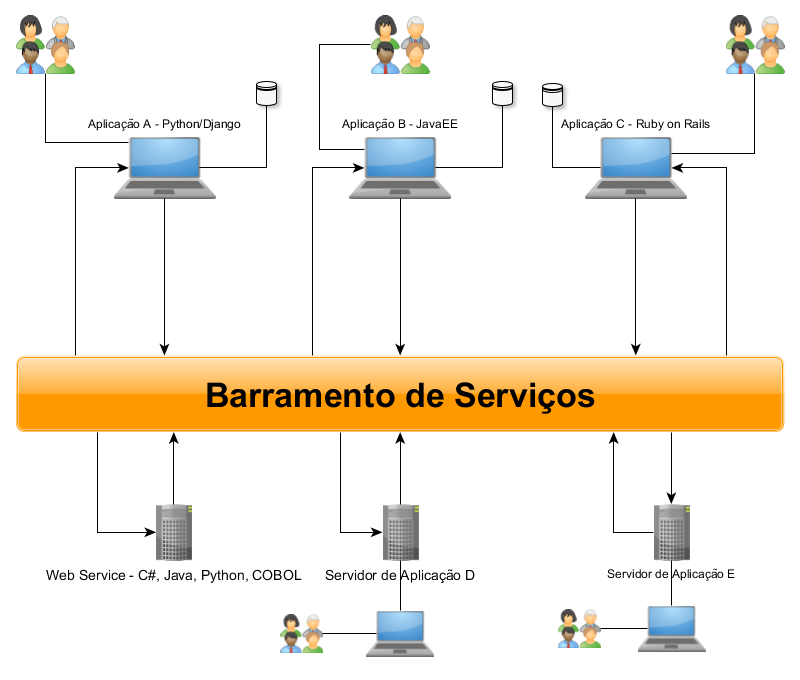
\includegraphics[width=1\textwidth]{figuras/barramento_interoperabilidade.PNG}
\caption{Interoperabilidade em uma arquitetura baseada no modelo SOA.}
\label{barramento_interoperabilidade}
\end{figure}

A figura acima visa demonstrar a interoperabilidade em uma arquitetura baseada no modelo SOA: é possível inferir que as diversas aplicações fazem a requisição dos serviços disponíveis por meio do uso do barramento de serviços, que também pose ser interpretado como um barramento de aplicações. As aplicações podem ser desenvolvidas utilizando-se tecnologias e paradigmas distintos e a troca de dados entre elas se darão via mensagens de requisição e resposta entre as aplicações usuário, que requisitam operações dos serviços, e os serviços, responsáveis por processar as requisição e fornecer uma resposta.

A figura também exibe um fato interessante na arquitetura proposta: não é necessário que um serviço seja apenas um serviço hospedado em um servidor. As aplicações poderão operar tanto em modo \textit{standalones}, sendo executadas de forma independente dos outros serviços ou aplicações, quanto como um serviço para a plataforma virtual unificada ou para outras aplicações que tenham conhecimento da existência e do protocolo de uso deste serviço.

O ESB é uma ferramenta que fornece as funcionalidades do barramento de serviços. Seu irá garantir que, sempre que este estiver ativo, as requisições que serão realizadas sempre terão uma resposta, mesmo sendo algo que indique a inatividade do serviço requerido ou a não autorização para acesso à este. Ao adicionar um novo serviço à arquitetura utilizando o ESB, deverão ser especificados tanto os procedimentos quando uma nova requisição for feita quanto aqueles passos que conduzem ao envio de uma resposta de acesso ao serviço especificado, sendo esta resposta advinda do próprio serviço ou uma resposta padrão, também especificada, em caso de falha ou sucesso ao executar a requisição.

Com base nos requisitos essenciais levantados e no estudo realizado sobre o modelo arquitetural SOA, o modelo proposto pode ser visto na imagem abaixo:

\begin{figure}[htb]
\centering
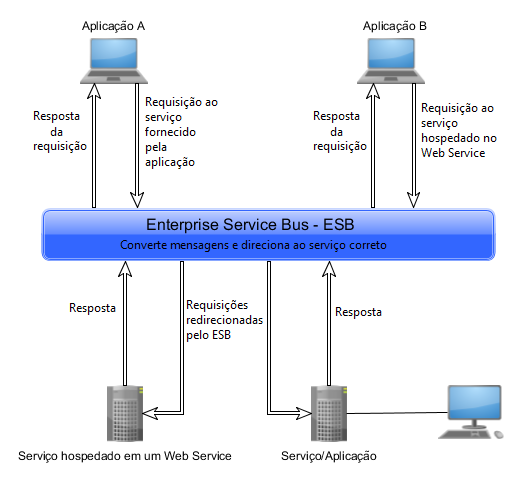
\includegraphics[width=0.8\textwidth]{figuras/uso_esb.PNG}
\caption{Proposta da arquitetura baseada no modelo SOA com o uso de um ESB.}
\label{uso_esb}
\end{figure}

A comunicação entre aplicações e serviços deverão seguir o padrão de protocolo também definido neste documento, afim de manter uma regra de execução na troca de informações. O protocolo também facilitará a adição de um novo serviço à arquitetura no que diz respeito aos procedimentos de transformação dos dados e adaptação entre tecnologias e protocolos de comunicação adotados.

\subsubsection{Ferramentas ESB}
Existem diversas ferramentas deste tipo disponíveis e em uso por grandes organizações, tais como JBoss ESB, Mule ESB, Zato e WSO2 ESB. Algumas destas ferramentas já foram levantadas, e, sendo o ESB um elemento importante para a implementação aqui porposta, uma análise destas ferramentas com junto a uma avaliação baseada em critérios ainda não estebelecidos a fim de eleger uma ferramenta deste tipo para apoiar o desenvolvimento do trabalho.

\subsection{Protocolo de comunicação}

{DESCREVER O PROTOCOLO, JUSTIFICAR O USO E ESTABELECER OS PADRÕES A SEREM UTILIZADOS}
--- USAR O REST E DESCRVER COMO ELE VAI SER UTILIZADO, QUAL O PADRÃO ESTABELECIDO DO PROTOCOLO, Formato de mensagens,  DESENHAR O DIAGRAMA DE SEQUENCIA E TALS---

\section{Metodologia}


\section{Cronograma de execução}
Para o desenvolvimento da proposta e completude da memsa com sucesso, foram criados dois cronogramas distintos para as fases de estudo e elaboração da proposta e para a fase de prova de conceito e implementação da proposta desenvolvida. Os cronogramas contém a descrição das atividades realizadas, bem como os prazos relacionados a cada atividades e podem ser visualizados nas tabelas abaixo.

\begin{table}[!h]
\centering
\caption{Cronograma de atividades relacionadas ao TCC 1}
\label{cronograma_tcc1}
\begin{tabular}{|p{9cm}|c|c|c|c|c|c|}
\hline
Atividade                                                   & \multicolumn{1}{l|}{Jan} & \multicolumn{1}{l|}{Fev} & \multicolumn{1}{l|}{Mar} & \multicolumn{1}{l|}{Abr} & \multicolumn{1}{l|}{Mai} & \multicolumn{1}{l|}{Jun} \\ \hline
Identificação da necessidade                                & X                           &                             &                              &                            &                             &                              \\ \hline
Leituras sobre modelos arquiteturais                        & X                           &                             &                              &                            &                             &                              \\ \hline
Pesquisa sobre o modelo arquitetural mais adequado          & X                           & X                             &                              &                            &                             &                              \\ \hline
Pesquisa sobre trabalhos relacionados                       & X                           & X                        &                              &                            &                             &                              \\ \hline
Levantamento superficial de ferramentas ESB                 &                             & X                        & X                            &                            &                             &                              \\ \hline
Organização das referências                                 &                             &                             & X                            &                            &                             &           \\ \hline
Escrita formal da proposta                                  &                             &                             &                              & X                          &                             &           \\ \hline
Estabelecimento de metodologia                              &                             &                             &                              & X                          &                             &             \\ \hline
Escrita do TCC 1                                            &                             &                             &                              &                            & X                           & X          \\ \hline
\end{tabular}
\end{table}

\begin{table}[!h]
\centering
\caption{Cronograma de atividades relacionadas ao TCC 2}
\label{cronograma_tcc2}
\begin{tabular}{|p{9cm}|c|c|c|c|c|c|}
\hline
Atividade                                                   & \multicolumn{1}{l|}{Jul} & \multicolumn{1}{l|}{Ago} & \multicolumn{1}{l|}{Set} & \multicolumn{1}{l|}{Out} & \multicolumn{1}{l|}{Nov} & \multicolumn{1}{l|}{Dez} \\ \hline
Análise de ferramentas a serem utilizadas                   & X                           &                             &                              &                            &                             &                              \\ \hline
Implantação da ferramenta escolhida                         &                             & X                            &                              &                            &                             &                              \\ \hline
Adaptação de uma aplicação já desenvolvida                  &                             &                               & X                            &                            &                             &                              \\ \hline
Implementação do uso da ferramenta com a aplicação adaptada &                             &                         &                              & X                          &                             &                              \\ \hline
Escrita do TCC 2                                            &                             &                             &                              &                            & X                           & X          \\ \hline
\end{tabular}
\end{table}